\chapter{Calibration and digitisation}\label{ch:ADC}

\section{Temperature sensor} \label{sec:ADCTemp}

	\subsection{Analytical Design} \label{sec:ADCTempAna}

Equation \ref{eq:temp} for the sensor voltage and \ref{eq:amp} for the amplifier, where the addition of a virtual ground and offset correction are combined by $V_{offset}$.

\begin{equation}
\vspace{-0.4cm}
\label{eq:temp}
V_{sense} = V_{0} + \alpha(T) \;\;\; \rightarrow \;\;\; T = \frac{1}{\alpha}(V_{sense} - V_{0})
\end{equation}

\begin{equation}
%\vspace{-0.4cm}
\label{eq:amp}
V_{out}=A_{v}\left({V}_{sensor}-{V}_{offset}\right) \;\;\; \rightarrow \;\;\; {V}_{sensor} = \frac{V_{out}}{A_{v}} + V_{offset}
\end{equation}

Combining \ref{eq:temp} and \ref{eq:amp} gives

\begin{equation}
\label{eq:comb}
T = \frac{V_{out}}{\alpha A_{v}} + \frac{V_{offset} - V_{0}}{\alpha} = 1.6(V_{out}) + 34
\end{equation}

for $V_{0} =$ \SI{440}{mV}, $\alpha =$ \SI{35}{mV}, $V_{offset} =$ \SI{1.63}{V}, $A_{v} = 17.86$. For an ADC:

\begin{equation}
\label{eq:adc}
\mathrm{ADC} = (2^{10}-1)\frac{V_{in}}{V_{ref}} \;\;\; \rightarrow \;\;\; V_{in} = \frac{\mathrm{ADC}(V_{ref})}{2^{10}-1}
\end{equation}

\ref{eq:adc} into \ref{eq:comb}, with $V_{out}$ as ADC input, converts the sampled ADC value to temperature output: 

\begin{equation}
\vspace{-0.4cm}
\label{eq:adctemp}
T = (1.6)\frac{\mathrm{ADC}(V_{ref})}{2^{10}-1} + 34
\end{equation}



	\subsection{Empirical Design} \label{sec:ADCTempEmp}
\begin{wrapfigure}{r}{0.5\textwidth}
\centering
\vspace{-0.6cm}
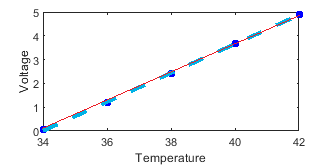
\includegraphics[width=0.5\textwidth]{./Figures/linreg}
\caption{Voltage against temperature}
\label{fig:linreg}
\end{wrapfigure}
Simulation yields the data points in figure \ref{fig:linreg}. Linear regression results the empirical equation \ref{eq:linreg}, graphed in light blue, which is implemented in software as to provide a digital temperature reading - see pseudocode below. Equation \ref{eq:adctemp} corresponds closely to the analytical equation \ref{eq:comb}, graphed in red. Python implementation yields a 1\degree C temperature reading accuracy for the full input range. 
 
\begin{equation}
\label{eq:linreg}
T = 1.644985924\left(V_{out_{avg}}\right) + 33.92887739
\end{equation}

Pseudocode:
\begin{algorithm}
V\textunderscore avg = V\textunderscore out / length(V\textunderscore out)\\
T = 1.644985924*V\textunderscore avg + 33.92887739
\end{algorithm}





\vspace{-0.7cm}
\section{Heart rate sensor}
\label{sec:ADCHeart}


	\subsection{Analytical Design} 					\label{sec:ADCTempAna}
The heart-rate signal consists of square wave pulses of which the periods correspond to the heart-rate. 



	\subsection{Empirical Design} 					\label{sec:ADCTempEmp}

Include flow diagram of code or pseudocode as a list.
No need to include the 10-bit ADC in this section. 
